\chapter{Adaptive Learning}
\label{chap:adaptive-learning}

% TODO:
% - incorporate other notes from my/thesis gdoc
% - inspiration from relevant articles
% - add references for provided examples (playing chess, autonomous car, ...)

From playing chess to driving an autonomous car,
  artificial intelligence proved to be a mighty tool
  for tackling difficult algorithmic tasks.
The power of artificial intelligence can be also used
  to develop a personalized adaptive system for learning programming.
Such system would create an optimal learning experience for each student
  by providing them with problems of difficulty matching their skill,
  so that the student stays challenged and interested in solving them.

In the existing systems (\ref{sec:existing-systems}),
  the sequence of tasks is the same for everybody.
As a result, the progress is necessarily too slow for some students,
  who could skip some of the tasks,
  while being too fast for others,
  who could highly benefit from solving a couple of other similar tasks.
Artificial intelligence can be used to personalize
  the sequence of tasks for every student.
By giving the student a suitable task
  -- neither too easy, nor too difficult --
  it can help the student to get into the state of flow
  (\ref{sec:motivation.challenge}).

In addition to choosing the most suitable task for given student,
  artificial intelligence has also other possible uses in learning systems,
  for example automatic hints generation \cite{generating-hints}
  or skills visualization (TBA: ref).
Furthermore, artificial intelligence techniques can be used
  to analyze collected data offline.
Such analyses can reveal problematic tasks,
  or suggest how to group tasks into categories (TBA: ref).

Adaptive learning systems have been already successful in some domains.
For instance, Map Outlines%
  \footnote{Available at \url{https://outlinemaps.org}.},
  developed by Adaptive Learning research group at Masaryk University,
  is an intelligent web application for learning geography.
It has been used by tens of thousands of students
  and online experiments have confirmed
  that the adaptivity of the system helps to improve the learning outcome
  \cite{alg.evaluation-geography}.
In addition to geography, similar adaptive web applications
  for learning anatomy%
  \footnote{Available at \url{https://practiceanatomy.com}.},
  biology%
  \footnote{Available at \url{https://poznavackaprirody.cz} (in Czech only).},
  elementary mathematics%
  \footnote{Available at \url{https://matmat.cz} (in Czech only).},
  and Czech grammar%
  \footnote{Available at \url{https://umimecesky.cz} (in Czech only).},
  were developed by the research group in recent years.

Section \ref{sec:student-modeling} presents how to model students
  in the context of learning programming.
Sections \ref{sec:task-recommendation} and \ref{sec:mastery-learning}
  then describe how to use these models to make a learning system adaptive.
Finally, section \ref{sec:metrics-and-evaluation} discusses how to evaluate
  different models or even whole learning systems.


\section{Student Modeling}
\label{sec:student-modeling}

For the system to be adaptive, models of
  a student skill, task difficulty, and student-task interaction
  need to be designed, implemented, and evaluated using collected data.
The purpose of these models is to predict the probability that a given student
  would solve a given task
  and also the time the student would need to complete the task.


\subsection{Data}
\label{sec:student-modeling.data}

To learn model parameters, such as difficulty of individual tasks, some data is needed.
What data and how much data is needed differs across models.
Some data about tasks are independent of students;
therefore, they can be obtained in advance,
which can be useful for initial task difficulties estimates.
Three types of task data are distinguished:

\begin{itemize}
  \item task statement (including name and world description),
  \item sample solution (or multiple solutions),
  \item expert labels (e.g. covered concepts).
\end{itemize}

Task statements are always available,
  because they are needed to present tasks to students.
However, obtaining sample solutions and expert labels
  incurs additional costs for a new system.
% TODO: Note that quite often, systems needs sample solutions and some labels
%       for the presentation purposes anyway.
Moreover, they can be noisy and imperfect.
For example, an annotator can forget to include some labels
  or even make a mistake in the sample solution.

Once the task is deployed in the running system,
  rich data can be collected from each interaction between a student and a task:
\begin{itemize}
  \item whether the task was eventually solved,
  \item solving time,
  \item number of clicks, number of code executions,
  \item program snapshots (e.g. after each code change),
  \item rating or labels provided by the student (e.g. perceived difficulty).
\end{itemize}

% TODO: also consider to include hints in the list
% TODO: mention different granularity levels for taking program snapshots (+cite)

\subsection{Item Response Theory}
\label{sec:irt}

The simplest version of item \emph{item response theory} (IRT)
  \cite{irt-visual-guide}
  models each student by a one-dimension skill $s$,
  and each task by a one-dimension difficulty $d$.
IRT assumes that the probability of a student with skill $s$
  successfully solving a task with difficulty $d$
  is given by the following function:
  \begin{equation}\label{eq:logistic}
  P(s, d) = \frac{1}{1 + e^{-(s - d)}}
  \end{equation}

% TODO: mention 2-parameter model (explain discrimination parameter)
\begin{figure}[h]
  \centering
  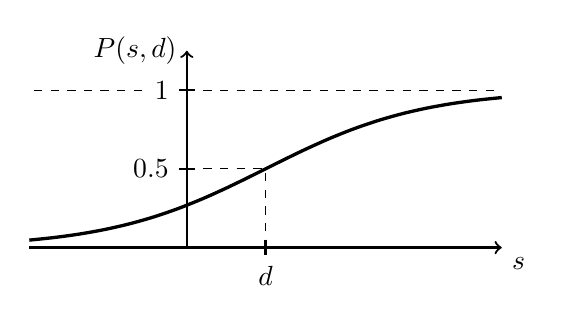
\begin{tikzpicture}[domain=-2:4, smooth, samples=20, scale=1]
  \draw [thick, ->] (-2,0) -- (4,0) node [below right] {$s$};
  \draw [thick, ->] (0,0) -- (0,2.5) node [left] {$P(s,d)$};
  \draw [thick] (-0.1,1) node [left] {$0.5$} -- (0.1,1);
  \draw [thick] (-0.1,2) node [left] {$1$} -- (0.1,2);
  \draw [thin, dashed] (0,2) -- (4,2);
  \draw [thin, dashed] (0,1) -- (1,1) -- (1, 0);
  \draw [thin, dashed] (-0.57,2) -- (-2,2);
  \draw [thick] (1,0.1) -- (1,-0.1) node [below] {$d$};
  \draw [very thick] plot (\x, {2 / (1 + exp(1 - \x))});
  \end{tikzpicture}
  \caption{One-parameter Unidimensional Logistic Model}
  \label{fig:logistic-model}
\end{figure}

This basic model was originally developed for a simple knowledge testing
  and therefore it assumes a single constant skill.
However, programming skill is multidimensional;
  for example, one student can be proficient with functions and struggle with loops,
  while another student can master loops and struggle with functions.
Furthermore, these skills should be ideally changing significantly during
  the interaction with the system, because students are learning.

Another drawback of the IRT is that it only uses
  the binary data about successes and failures.
As nearly all interactions in programming learning systems end with a solved task,
  it would be more useful to work with solving times,
  which can provide more information about students' skills.

Item response theory can be extended to overcome these limitations.
\emph{Problem Response Theory} (PRT)
\cite{alg.problem-response-theory, pelanek-student-modeling-times}
% TODO: only cite the more relevant paper (or extend this section and cite both
% on relevant places)
predicts problem solving times instead of probability of success,
assuming an exponential relationship between a problem solving skill
and the time to solve a problem.
PRT can be formulated to use multidimensional skills.
The model parameters (skills and difficulties) can can be estimated from the data
  using one of the \emph{maximum likelihood estimation} algorithms.
  % TODO: cite paper describing the parameters estimation (or MLE?)
% (for IRT, it's \cite{irt-theory-and-practice}, but PRT would be better)

% TODO: find and provide the details about the learning extension of PRT
% (isn't it already the elo?)

% TODO: Add note that the assumption of exponential relationship is justified
% by observed solving solving times distribution and it is also intuitively
  % plausible - multiplicative nature of solving times.



\subsection{Elo}
\label{sec:elo}

The Elo model \cite{alg.elo}
  extends the logistic model presented in section \ref{sec:irt}
  to capture changing knowledge.
Inspired by the rating of chess players \cite{elo-rating},
  the model interprets each attempt  to solve a task
  as a ``match'' between the student and the task.
After this match ends, skill and difficulty estimates are revised.

If the student solves the task faster than expected by the model,
  their skill is increased and the difficulty estimate of the solved task is decreased.
On the contrary, if the student fails to solve the task or if takes them too long,
  their skill is decreased and the difficulty estimate of this task is increased.

% TODO: formulas (for time-variant of elo)
% TODO: mention differnet updates for tasks (exponentially decayed) and
% students (their skill is assumed to change and not converge)

The main advantage of using the Elo model is its simplicity, flexibility,
  good performance and intrinsic online nature, which allows for immediate
  updates of parameters as students are interacting with the system.

% TODO: include other models, PFA, BKT etc.


\subsection{Concepts}

% TODO: consider to move this section before the description of individual
% models
% TODO: fix and mention used terminology: concept vs. skill

A vast amount of research in the field of adaptive learning
  restricts its attention to a one-dimensional skill.
This assumption is reasonable for many logic puzzles (e.g. sudoku);
however, solving programming tasks requires multiple diverse skills,
  such as loops, conditional commands, or functions.
It is possible to master loops while struggling with functions,
  and vice versa.

As mentioned in sections \ref{sec:irt} and \ref{sec:elo},
  both the IRT and Elo models can be extended to work with multidimensional skills.
% TODO: However, the way they compose multiple skills into a single prediction
% is not completely justified / can differ depending on domain/skills (e.g.
% adding skills vs taking best/worse)
Although modeling multiple skills seems useful,
  there is a trade-off between the complexity of the model (number of skills)
  and how well (or how fast) the parameters can be estimated.
More parameters require more data and time for the estimates to converge.
% TODO: which is especially concern for students; 1. predictions needed
% immediately for new students (no/little data), 2. students' skills are
% assumed to change (tasks didn't have these problems)


% \subsection{Learning Concepts from Data}

Concepts can be either defined manually or detected automatically
  \cite{niznan-thesis}.  % TODO: specify chapter/pages
Manually selected concepts, such as loops and conditional commands,
  have the advantage of being interpretable,
  so they can be used for skills visualizations in the user interface
  to provide students with the information about their learning progress.
Furthermore, no data needs to be collected in advance,
  while the automatic techniques require a lot of data to provide stable results.  % TODO: how much?


% \subsection{Prerequisites}
Undoubtedly, there are some relationships between skills;
  for example, nested loops cannot be mastered without mastering simple loops.
The hierarchical structure between concepts can be modeled
  as a directed acyclic graph (DAG),
  where each vertex is a concept and each edge represents a prerequisite.
Having DAG of concepts then allows to model students using Bayes networks
  \cite{its-programming}.

% TODO: simple diagram: DAG of concepts example

\section{Task Recommendation}
\label{sec:task-recommendation}

Student models are used by an \emph{instructional policy} to recommend
  the most suitable task for a student.
In spite of having all the predictions about success probabilities
  and time estimates available,
  task recommendation is not an easy task.
First, it is not clear what difficulty level is optimal.  % TODO: example (75 % of success etc.)
Second, it may vary for different students, domains or types of problems.
Furthermore, optimal difficulty is not the only criterion to be considered.
For instance, diversity of tasks is important to keep students interested.
No principled techniques for task recommendation have been developed yet;
however, several heuristic approaches have been used
  and proved to work well (TBA: ref).

Task recommendation is not a necessary requirement
  for the system to be adaptive.
Student models can be utilized by other means to achieve personalized behavior,
  e.g. in mastery learning (section \ref{sec:mastery-learning}).
The system can also just provide students with predicted solving times
  and let them to choose the next task they want to solve.

Showing predictions can be already perceived as a very mild form of recommendation.
Indeed, recommendations can range from \emph{soft} to \emph{hard}.
Soft recommendations can be achieved either by
  ordering tasks according to suitability,
  filtering and only showing a subset of tasks,
  or showing suggestion such as
  ``too easy'', ``too difficult'' and ''ready to attempt'' next to each task.
For example, suggestions in the form of traffic-light colors
  are used in the system described in \cite{its-programming}.
The system can be more strict and show only a single recommended task,
  or even enforce the recommendation by immediately progressing student to
  the next task without asking and giving them a chance to select a different task.

\bigskip
\emph{TODO:\\details about techniques (heuristics, methods) for selecting single best task}

\section{Mastery Learning}
\label{sec:mastery-learning}

\emph{TODO:\\describe mastery learning + usage of student models%
(to show the progress and to determine that the student already achieved the mastery)}

% TODO: screenshot of a mastery progress bar (e.g. from UmimeX)

\section{Metrics and Evaluation}
\label{sec:metrics-and-evaluation}

To decide if the adaptivity of the system increases the learning outcomes,
  a suitable metric must be chosen and incorporated into the system,
  for example using pre-tests and post-tests.
Ideally, the system should also allow to easily change various conditions
  for subsets of students and hence perform controlled online AB experiments.


\subsection{Metrics for Predictions}

\emph{TODO}

%TODO: data we need -- this is simple: we can collect the objective solving times and compare
%with predictions (there is some noise, because of students taking breaks, cheating, etc., but should be ok)
%
%TODO: mention standard metrics and evaluation methodologies in ML (for
%predicted times, RMSE vs. MAE etc.)


\subsection{Metrics for Recommendation}

\emph{TODO}

%TODO: what data to use? much less clear than  for predictions
%
%TODO: mention standard metrics and evaluation methodologies in RC (for recommended tasks)
%
%The tasks environment in learning systems often differ significantly
%  from the real-world environment,
%  e.g by using blocks instead of text
%  and other aspects mentioned in section \ref{sec:strategies-for-easier-learning}.
%This makes evaluation harder, because while the collected data on which we
%  evaluate the system comes from the system itself,
%  ultimately students leave this simplified environment
%  and the performance outside the learning system is the important criterion.

% This issue is mentioned in \cite{challenges-of-blocks-based-environments},
% by Werntrop and Wilensky
% in the context of proper evaluation of block-base programming environments.

% TODO: this relates to next subsection on ultimate goal vs. proxy metrics
% TODO: also consider short discussion on high-level vs. low-level goals
% (also known as mission/purpose/vision vs goals, or goals vs means
% and discussion on goals vs metrics



\subsection{Ultimate and Proxy Metrics}

\emph{TODO}

%TODO: explain possible metrics derivation: -- with specific example of learning programming
%1. from the ultimate goal (vision, mission) -- but make it precise to make it evaluable (if had all the data we need)
%2. proxing 1 to make it measurable in the long term (AB experiment)
%3. proxing 2 to make it measurable in the short term (live evaluation)
%4. proxing 3 to make it work with offline data (to learn hyperparameters + for holdout evaluation)
%5. proxing 4 to make it differentiable function (to guide learning, ie. for updates after new s-t interaction)



\subsection{Perceived Flow}

\emph{TODO}

%Instead of using objective (factual, measured) data (such as solving time),
%we can ask students to provide explicit ``rating'' (subjective/perceived difficulty),
%  e.g. by selecting tags after solving a task,
%  such as ``too easy'', ``too difficult'', `just right''
%  (or possibly even more specific such as ``boring'', ``weird'', ``fun'').
%Advantage: flow looks as a good proxy metric to optimize.
%Disadvantages:
%  bother students with another questions,
%  takes time (but this is negligible comparing to solving programming task),
%  inaccurate (noise depending on the mood etc.)
%


\subsection{Iterative Improvement}
\label{sec:iterative-improvement}

\emph{TODO}


%TODO: explain importance of offline analysis and monitoring;
%TODO: the term ``human in the loop'' \cite{stupid-tutoring-systems-intelligent-humans}
%TODO: AB experiments
%TODO: importance of iterative improvement, rule of the loop;
%TODO: provide more details -> extend to a section
